\part{Design, Implementation and Extending the AMAS4Opt Building Blocks}

The work presented in this thesis is part on the ongoing ID4CS project. ID4CS (\emph{Integrated Design for Complex Systems}) funded by the French \emph{Agence Nationale de la Recherche} (National Research Agency)\footnote{COSINUS program, ANR-09-
COSI-005 reference} and involves nine partners, both from the academic and industrial work. The goal of the ID4CS project is to use the MAS approach to provide new tools for the design of complex systems. Our industrial partners, Airbus and Snecma, are involved in aeronautical design, and are thus fully concerned by the problematic of complex continuous optimization for system design.

For this reason, one of our concerns was not only to propose a new approach for continuous optimization, but also to put this approach in practice by integrating it into a working prototype which could be used by our partners. To this end we worked with our partners, including optimization specialists and software development experts, to propose such a tool, basing ourselves upon the ADELFE method. This method aims to guide the development of AMAS-based softwares from high level user requirements to the implementation nuts and bolts. Using ADELFE we made a comprehensive analysis of the domain and actors involved in the use of such a tool.

We also use the design tools provided with ADELFE to instantiate our MAS and integrate it into the prototype. Among these tools, we used notably the recent MAY framework. The goal of MAY is to provide suitable abstractions as well as reusable software components for the development of agents and multi-agents systems. We contributed to the enrichment of its components library by developing a general and modular agent architecture consistent with the AMAS theory, notably by proposing a modular skill stack principle, where different skills can be composed to address specific requirements.

While such work could seems to concerns software engineering experts more than computer scientists, we will see how existing MAS oriented methods such as ADELFE are still too high-level to be successfully directly applied to any domain (and more so to continuous optimization) without an important agent expertise and extensive research work. We will detail how the scientific work we produced and presented in the previous part, especially the identification of various NCS[[s]] and the mechanisms to solve them, can be generalized into \enquote{building blocks}. These building blocks could then be reused to guide the design of other MAS in the domain of problem solving. This work places itself into a more general effort to provide a general reusable toolbox for assisting non experts in applying AMAS to the domain of optimization, under the name \emph{AMAS4Opt} (AMAS for Optimization).

\chapter{ADELFE and MAY Architecture}\label{ADELFE_chapter}

\section{Overview of ADELFE}

In section \ref{AMAS-ADELFE}, we succinctly presented ADELFE\footnote{\url{http:/www.irit.fr/ADELFE/}}, the method which has been proposed for the design of AMAS. In this chapter we get back in more details about this method and what benefits it provided for the design of our system. 

ADELFE is a method devoted to software engineering of adaptive multi-agent systems. It was initiated by a French government funded project lead by IRIT (see \url{http://irit.fr/ADELFE-Project} for details) and has been continuously  enhanced since. Like previously said, the name \enquote{ADELFE} is the French acronym for \enquote{toolkit to develop software with emergent functionality} (\textit{Atelier pour le DEveloppement de Logiciels à Fonctionnalité Emergente}).

The ADELFE method in itself is based on the Rational Unifed Process (RUP) and is defined following the Software Process Engineering Meta-Model (SPEM)  \cite{PiGl2004.1,BeCaGlPi2005.1}. Since its revision \cite{Ro2008.3}, it is composed of five \emph{Work Definitions} ($WD$), themselves decomposed in several \emph{activities} making use of UML as well as the AMAS-ML and muADL languages. An overview of the method is shown on \figurename{} \ref{ADELFE_phases}.

\begin{figure}
\centering
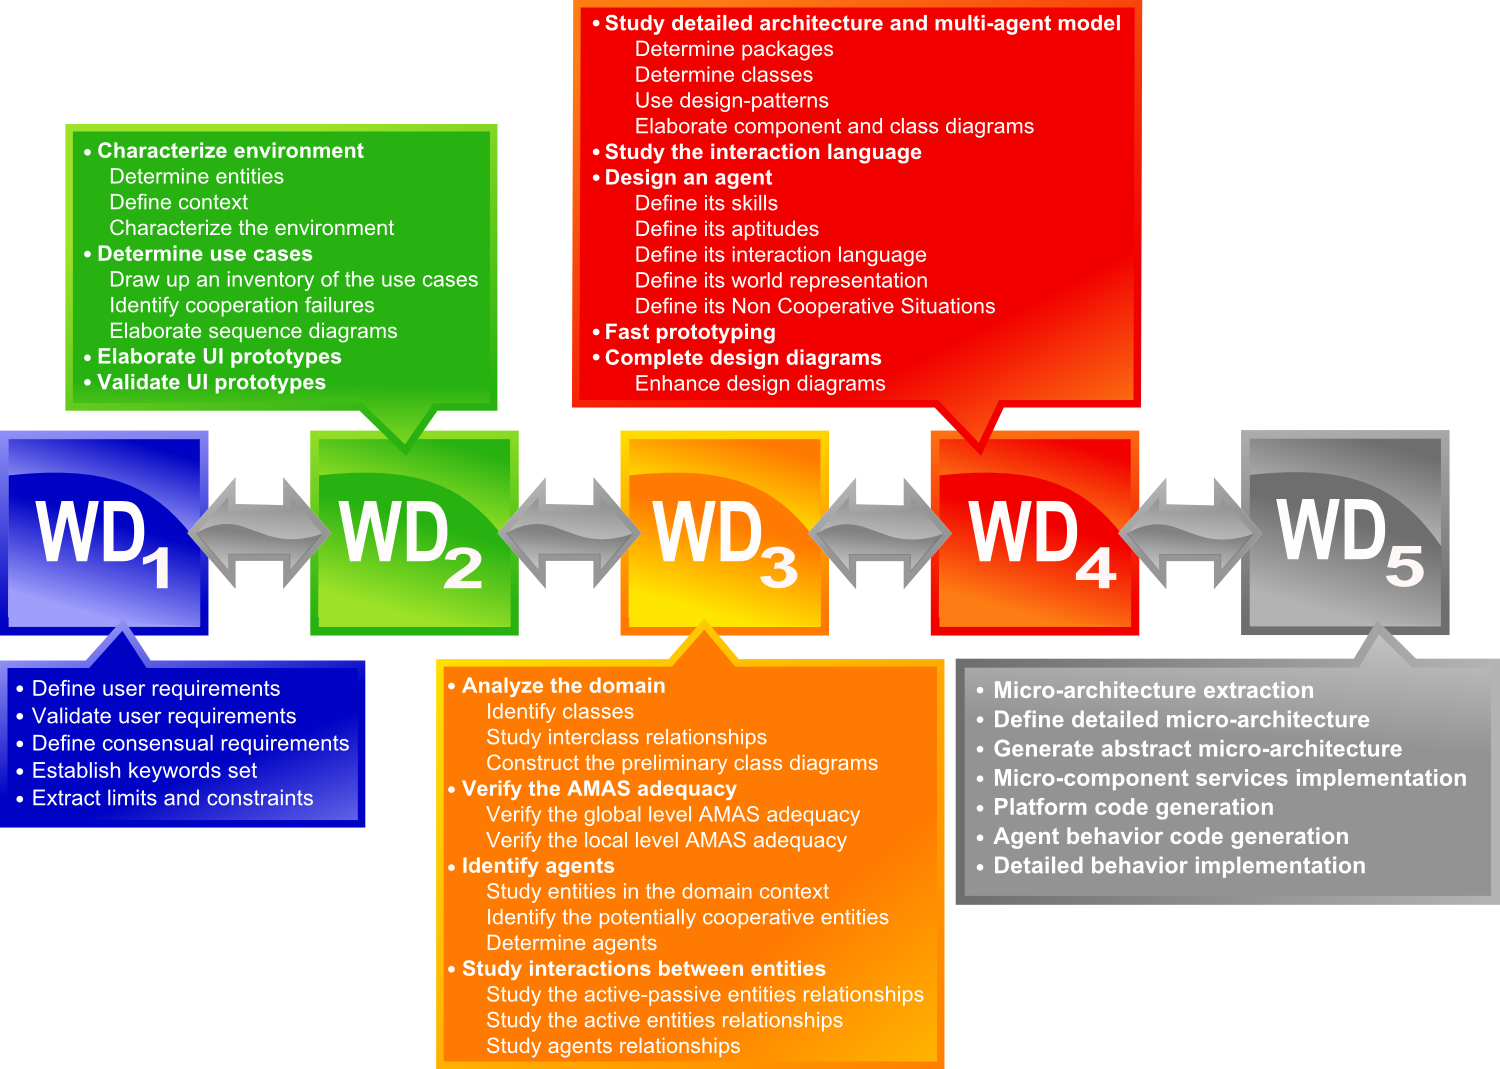
\includegraphics[width=\textwidth]{AdelfePhases}
\caption{Overview of the ADELFE Method}\label{ADELFE_phases}
\end{figure}

In regard of the RUP, ADELFE adds supplementary activities and roles which are specific to its approach for the design of AMAS compliant software.\\
The final requirement study ($WD_2$), was complemented with activities 6 and 7-2 concerning the characterization of the system environment and the identification of cooperation failures during the determining of the use cases. During the analysis ($WD_3$), additional activities 11 and 12 respectively check for the adequacy of AMAS to the problem and identify the agents involved in the system being built, while activity 13 is complemented with a step concerning the study of the relationships between agents. During the design ($WD_4$), activities 15 et 16 concerns the design of the system and the agents, while activity 17 concerning fast prototyping was added in order to be able to quickly test the proposed behavior of the agents. The development phase ($WD5$) concerns the architecture and the implementation of the agents and the system.

\section{The ID4CS Project: Applying ADELFE for the Design of a Continuous Optimization Tool}

[[TALK ABOUT ID4CS]]

Based on the guidelines of the ADELFE methodology we defined the requirements of the tool we proposed to develop. The following functionalities were identified:
\begin{compactitem}
\item Our tool will allow users to solve multidisciplinary optimization problems.
\item  The user will be able to load disciplinary models into the tool, express some constraints and objectives on these models and then use and interact with the tool to solve the defined problem.
\item Our tool will be reusable from one optimization problem to another in different application domains and will be a generic tool.
\item The user will be able to express uncertainties on some parts of the models or input variables.
\item The resolution will take into account these uncertainties.
\item The tool will be able to integrate well-known optimization techniques, and will allow the user to add new techniques to use during solving. The tool will also be able to interact with others optimization tools to ease the optimization process.

\item The user will be able (at runtime):
	\begin{compactitem}
    \item to monitor the system activity,
    \item to observe time history qualitative indicators,
    \item to adjust its parameters.
    \end{compactitem}
\end{compactitem}

\begin{figure}
\centering
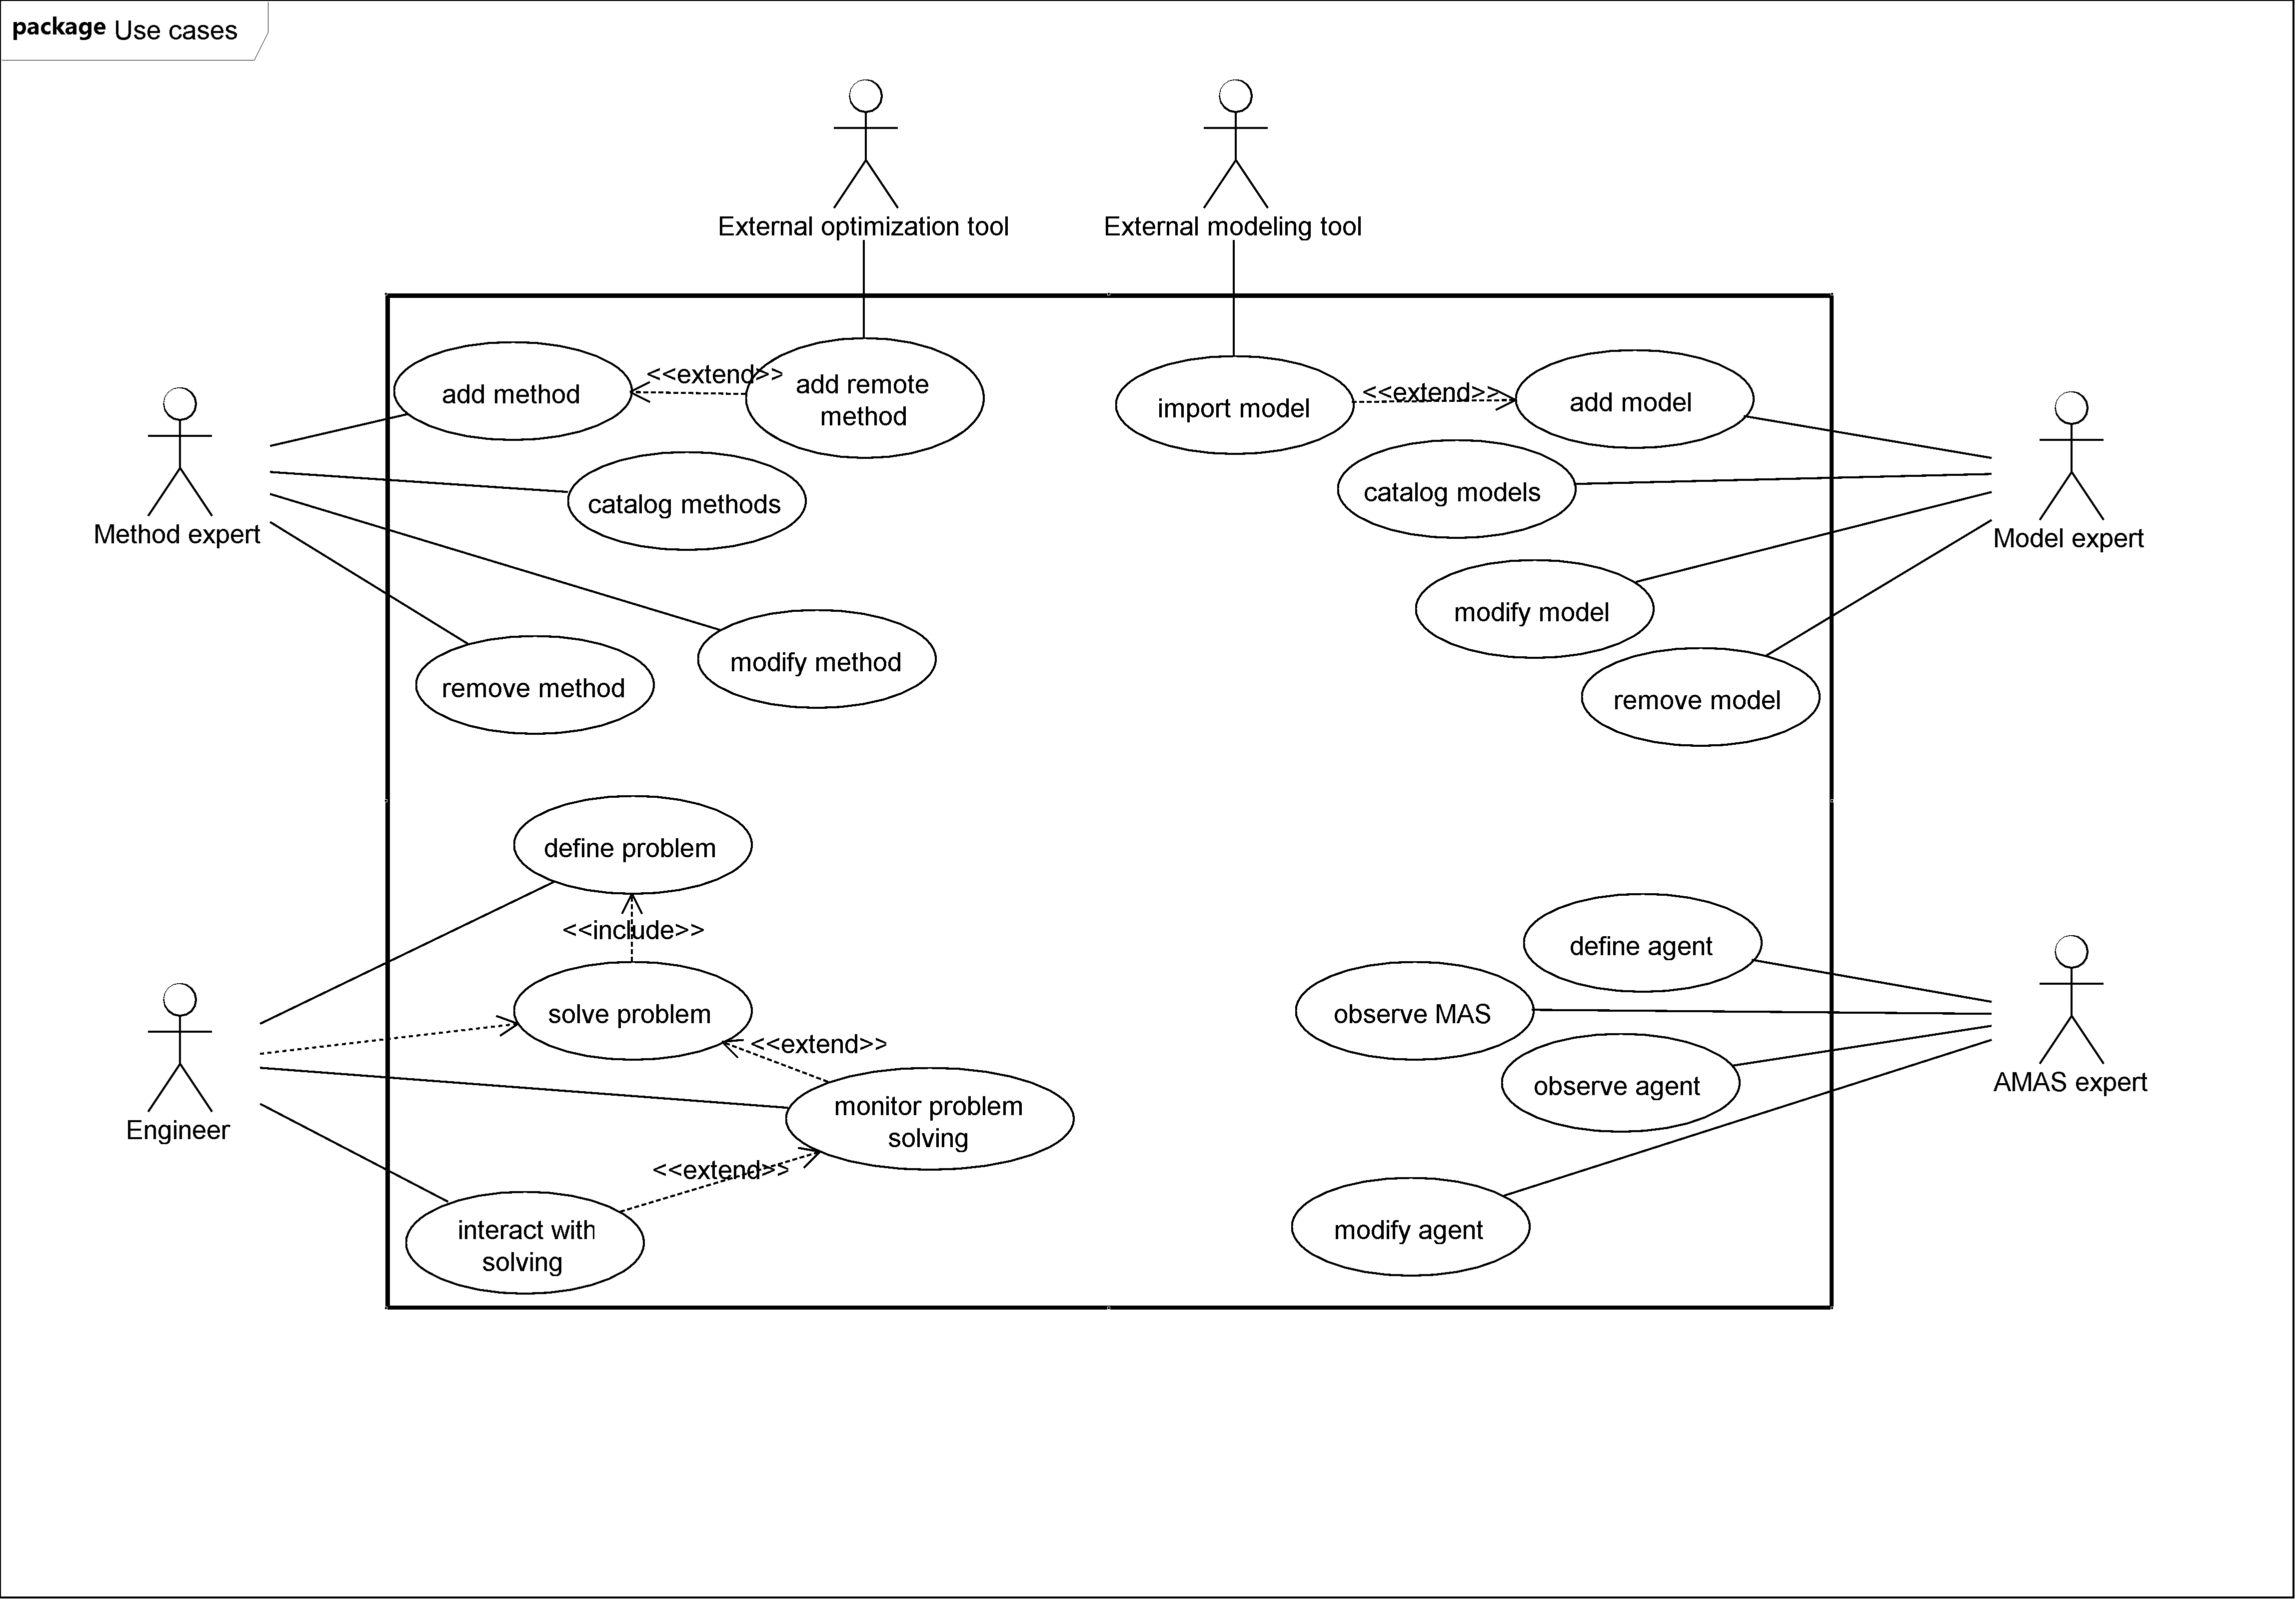
\includegraphics[width= \textwidth]{Use_cases}
\caption{Actors and use cases identified during requirements studies for ID4CS}\label{Use_cases}
\end{figure}

Several entities interacting with the tool were also identified. The \emph{Method expert} adds new optimization methods into the system. The expert field can be optimization methods (classic methods, AMAS methods ...) or uncertainties. The \emph{Model expert} adds new models into the system. The role of the \emph{Engineer} is to use the different elements defined by the other experts to define new problem for the system to solve and to monitor the functioning of the system. At last, the \emph{AMAS expert} has to define and tune the agents of the system. The system should also be able to integrate with external optimization and modeling tool, in order to accommodate the existing workflow and constraints of the users.

The different use cases which were identified for each of these entities are presented in \figurename{} \ref{Use_cases}.

The domain analysis (activity 10) roughly correspond to the work we provided in \ref{modeling}, as this activity correspond to the study of the application domain in interaction with the domain experts. The domain modeling roughly corresponds to an extended version of NDMO, with some additions and adjustments regarding the expected functionalities of the prototype. These adjustments concerns mainly the introduction of the \emph{workspace} and \emph{project} concepts, which allows the designer to organized its work, as well as the introduction of the external optimizer and uncertainties propagators as domain entities, in order to provide a more seamless integration of these tools into the prototype.\\
ADELFE then advocates an AMAS adequacy verification (activity 11), in which one checks using a set of questions if AMAS are a relevant solution for the problem to solve. We discussed at length in chapter \ref{AMAS_chapter} the advantages of the AMAS approach. Without much surprise the results of this activity were strongly in favor of using an AMAS solution, as the problem we aim to solve  is highly distributed, is not easily solvable by known algorithms, is potentially non-linear and evolving.

The next activities concerned the design of the agents themselves, their interactions, the identification and solving of the Non Cooperative Situations. The work concerning these activities is without much doubt the most difficult, involving in the ADELFE method the participation of an \enquote{agent designer}. Indeed, this part of the ADELFE method stays at a high abstraction level, and we can say without much controversy that the process of designing the agents is still highly exploratory, probably currently more related to a scientific study than to an engineering development. In this regard, our contribution presented in part \ref{MAS4Optim_part} provides the expected answers to these activities.

The last WD of ADELFE corresponds to the design of the agent architecture and implementation using MAY, the component-based framework developed in complement of ADELFE. While such framework aims ultimately to make the process as seamless and  automated than possible by providing reusable components, its early state implied once more some exploratory work on our part in order to produce, and in the end contribute to the MAY library with our own produced components. We will now see in the next chapter the architecture we proposed for a modular AMAS agent design.

\section{MAY Agent Architecture}

To implement the MAS, we used the Make Agents Yourself (MAY) framework  \cite{No2012.2}. MAY is a component-based framework that automatically generates an implementation of an agent architecture from a given description.

The ADELFE methodology proposes an abstract agent architecture (represented in \figurename{} \ref{AMAS-ML_agent}), which we translated into the MAY architecture description language, SpeADL. In the context of our study, as the agents communicate and interact only by messages passing we could make some simplifications in regard of the original modeling of communications and actions capability of the agents. All our agents use the same AMAS architecture. They are differentiated by specific implementations of the components. For example, \emph{Model} and \emph{Variable} agents will have different implementations of the \emph{Behavior} component.\\
The components of a MAY architecture are connected by \emph{ports}. A port can be though as a service interface, listing a set of available operations. Components expose lists of available and required ports. A component required ports must be linked to available ports provided by other components, satisfying these interfaces.

\begin{figure}
\centering
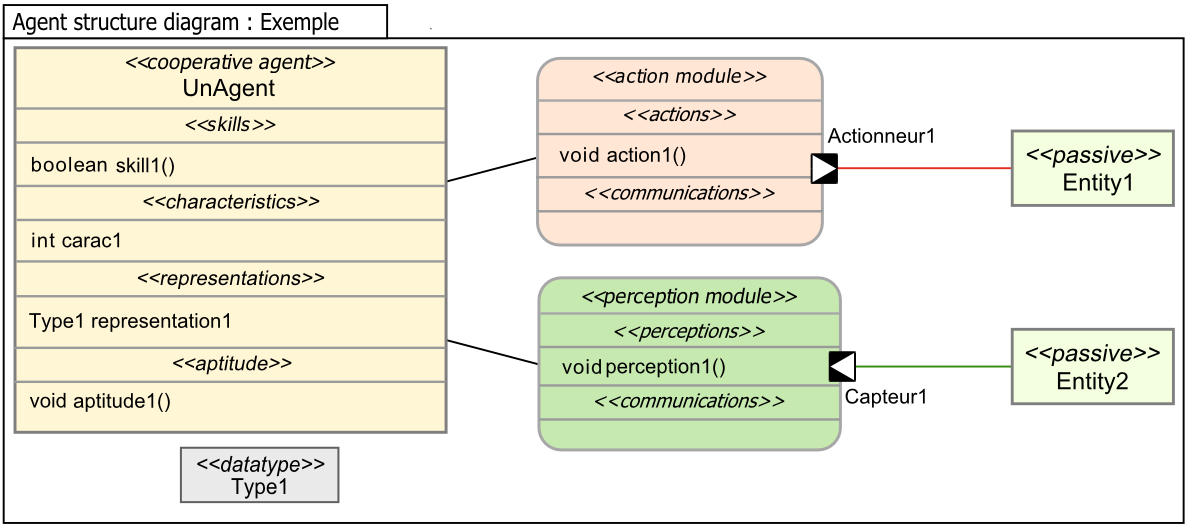
\includegraphics[width=\textwidth]{amasmlAgent}
\caption{AMAS agent architecture (as defined in ADELFE)}\label{AMAS-ML_agent}
\end{figure}

An illustration of this composition mechanism is shown on \figurename{} \ref{Speadl_example}. Two components $A$ and $B$ are present. The component $A$ exposes a port $P$ as available, which is required and used by the component $B$. Consequently, this last component is now able to call the operations declared by $A$ through this port, operations which are supposedly necessary for the good functioning of $B$. The way ports are used to connect otherwise independent components is in this way not too dissimilar to the role interfaces play in the context of \emph{dependency injection} design pattern.

\begin{figure}
\centering
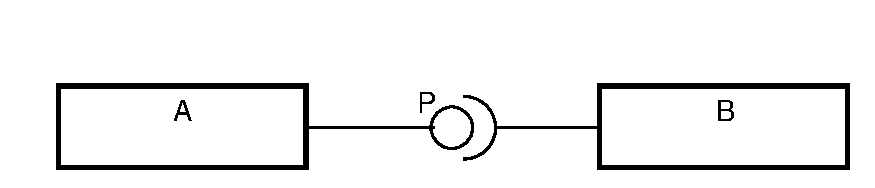
\includegraphics[width=0.4\textwidth]{Speadl_example}
\caption{Example of MAY composition}\label{Speadl_example}
\end{figure}

For the sake of clarity, the agent architecture is separated in three views: the \emph{behavior}, \emph{communication} and \emph{monitoring} views.

\subsection{Behavior}

The \emph{behavior} view (\figurename{} \ref{Arch-behavior}) contains the components related to the behavior of the agent. 

\begin{figure}
\centering
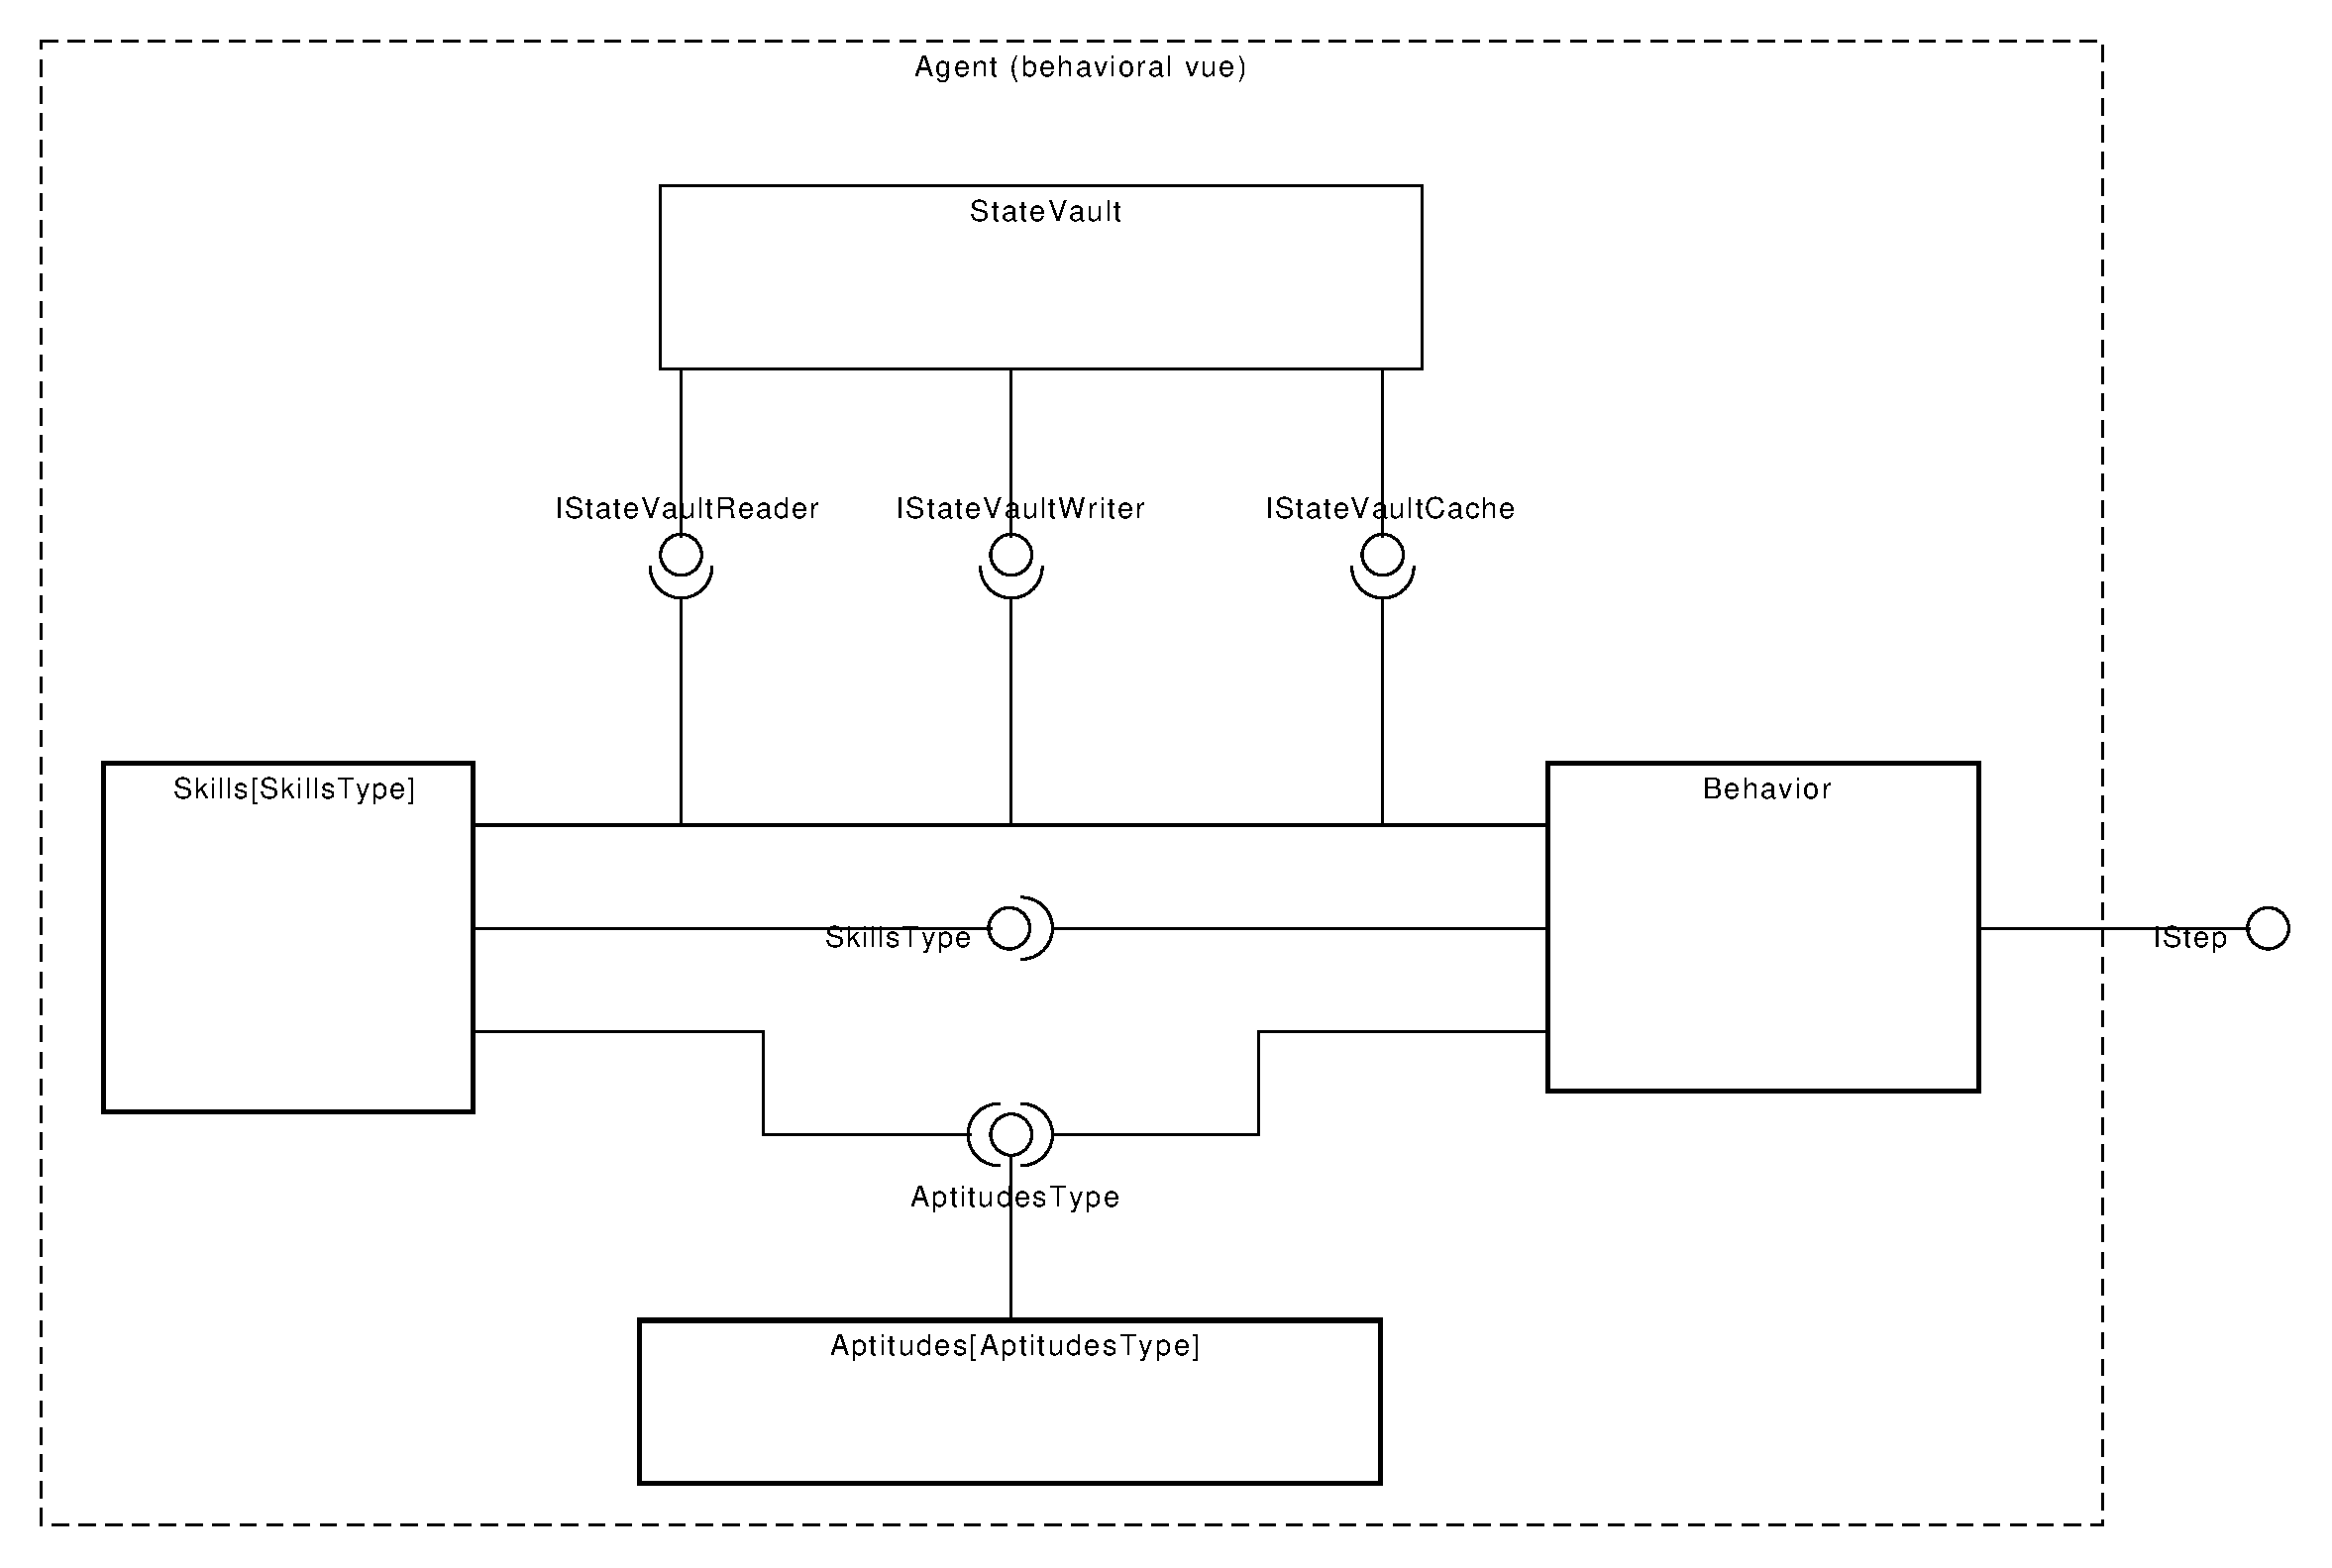
\includegraphics[width=0.6\paperwidth]{ID4CS_Speadl_behav}
\caption{Agent Architecture - Behavior view.}
\label{Arch-behavior}
\end{figure}

The \emph{Behavior} component contains the rules which dictate the behavior of the agent. This component can be seen as orchestrating the architecture. This component exposes to the outside of the environment the \emph{Step} port, which is used to make the agent execute a step. During a step the \emph{Behavior} component executes the agent rules. These rules will in return make use of the other components of the agent. [[RMK MPG: 1 exemple de règles cf 13.1 (??)]]

This behavior component contains the behavioral algorithms presented in chapter \ref{agent_behav_chap}. This component mostly contains the parts regarding the general steps of the agent behavior and making use of the more specialized methods  implemented in the \emph{Skills} and \emph{Aptitudes} components (for example, the exact computations involved in the detection of NCS).

The \emph{State Vault} contains the state of the agent. It is used by the components that need to save and read some state variables. Centralizing all the states variables into one component provides several benefits. First it is easier to save and restore the state of the agent, as we just need to save the content of the vault. It is also simple to share some data between components, as long as these components have access to the vault. And it is easy to provide a view of the agent state by just reading the State Vault.\\
This approach has however several drawbacks. It makes the code more verbose, as we need to explicitly read the value from the vault (and possibly store it to the vault if modified). It makes more difficult to track side-effects, as it is not obvious to know which component uses which value. At last there is sadly no way to strictly enforce that components only use the State Vault for storing state values, as neither Java nor MAY can provide such guarantee.

The \emph{Skills} component contains the skills of the agents. Each agent type has its own skills set, and skills can require to read and modify the agent state (thus the link between this component and the \emph{State Vault}). Some skills are used directly from the \emph{Behavior} rules but some skills can also be used by others skills.\\
Some examples of skills are: for a \emph{Variable agent}, the capability to change its value based on the requests it received and its old value. For a model agent, the capability to evaluate an internal model and get its output values.\\
Skills have the somewhat unique properties that they are in themselves stackable, depending on each others. To address this concern we propose to define the \emph{Skills} component itself as a complete components architecture in itself. We discuss this point in more details in section \ref{Skills_component_descr}.

The \emph{Aptitudes} component contains the aptitudes accessible to the agents. Unlike skills, aptitudes are general capabilities which do not rely on the state of the agent. Consequently, all agent types have access to the same aptitudes, and there is only one implementation of the \emph{Aptitudes} component.\\
Some aptitudes are used directly from the \emph{Behavior} rules but some aptitudes can also be used by skills or others aptitudes.
Some examples of aptitudes are: ordering a set of requests from the most to the least important. Make some manipulations on the potentially complex exchanged values (adding, calculate the norm etc., used for example in the manipulation of uncertain values).

The distinction between \emph{skills} and \emph{aptitudes} is not an easy one. The ADELFE method makes the distinction between the two concepts by defining skills to be capabilities of the agents inherent to its function, which cannot be abstracted from the application domain (for example the way a variable agent 
changes it value in response to the requests it receives), while aptitudes are more general \enquote{reasoning} capabilities, which could be reused between distinct systems (for example, using an Adaptive Value Tracker to track a value). The distinction between the two can be somewhat fuzzy, even more as often the firsts can depend on the seconds (for example, in the skill concerning the change of its value, the variable agent will use an AVT).\\
In our implementation, we choose to address this concern by classifying as skills the capabilities of the agents which are related (by using or modifying) the internal state of the agent, while classifying as aptitudes the capabilities which require no such things. Hence the distinction in our component modeling where the \emph{Skills} component requires an access to the internal state of the agent, while this requirement is absent from the \emph{Aptitudes} agent.

\subsubsection{Skills Component Architecture}\label{Skills_component_descr}

As stated, one of the more complex components of the agents is the one which encapsulate its skills. Indeed, each agent type has its own specific skills, and the skills in themselves can intervene at different levels or even be used by other skills. This specificity justifies the implementation of the internals of the \emph{Skills} component itself as component architecture. As skills are, by definition, specific to the application domain this modeling concerns more the explicit handling of the dependencies between \enquote{skillsets} than the reuse of the components. However, as some skills, while being specific to our application, are shared by several agent types. Based on the agent class diagram presented in \figurename{} \ref{SMA_class_diagram}, we derived the skills components tree presented in \figurename{} \ref{skills:graph}. As an example, \figurename{} \ref{skills:example} shows the composition of the \emph{Skills} component of a model agent.  As a remark, we see on the left figure that variable and output agents share the same skills. This pragmatic choice comes from the fact that, since the user can act on the problem at any time, a variable agent can become an output agent and \emph{vice versa}.

\begin{figure}[]
\centering
	\begin{subfigure}[b]{0.49\textwidth}
			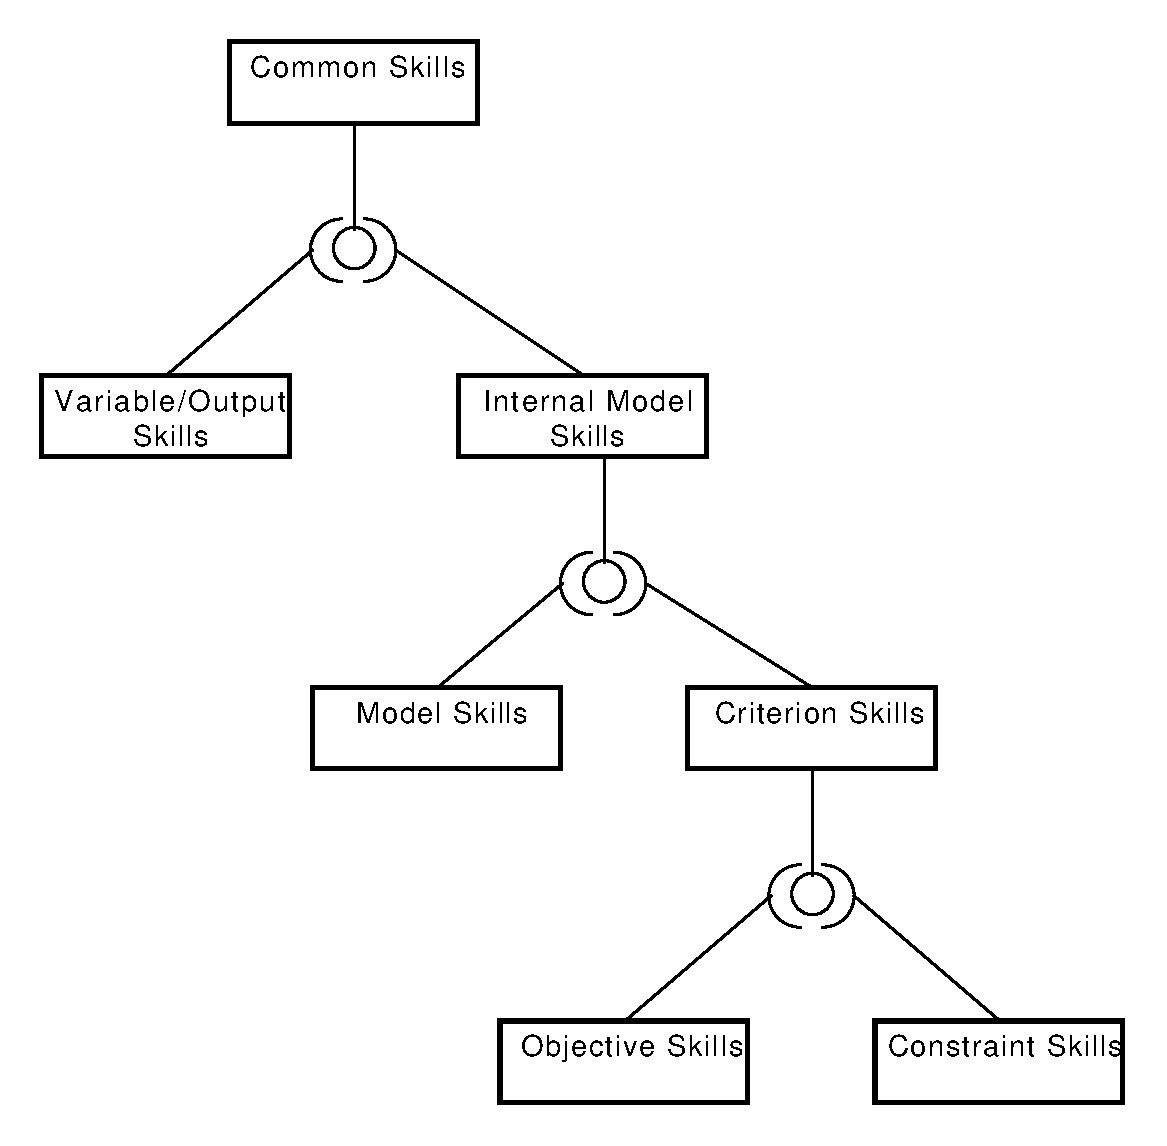
\includegraphics[width=\textwidth]{ID4CS_Speadl_skills}
			\caption{Skills components dependencies tree.}\label{skills:graph}
	\end{subfigure}
	\begin{subfigure}[b]{0.49\textwidth}
			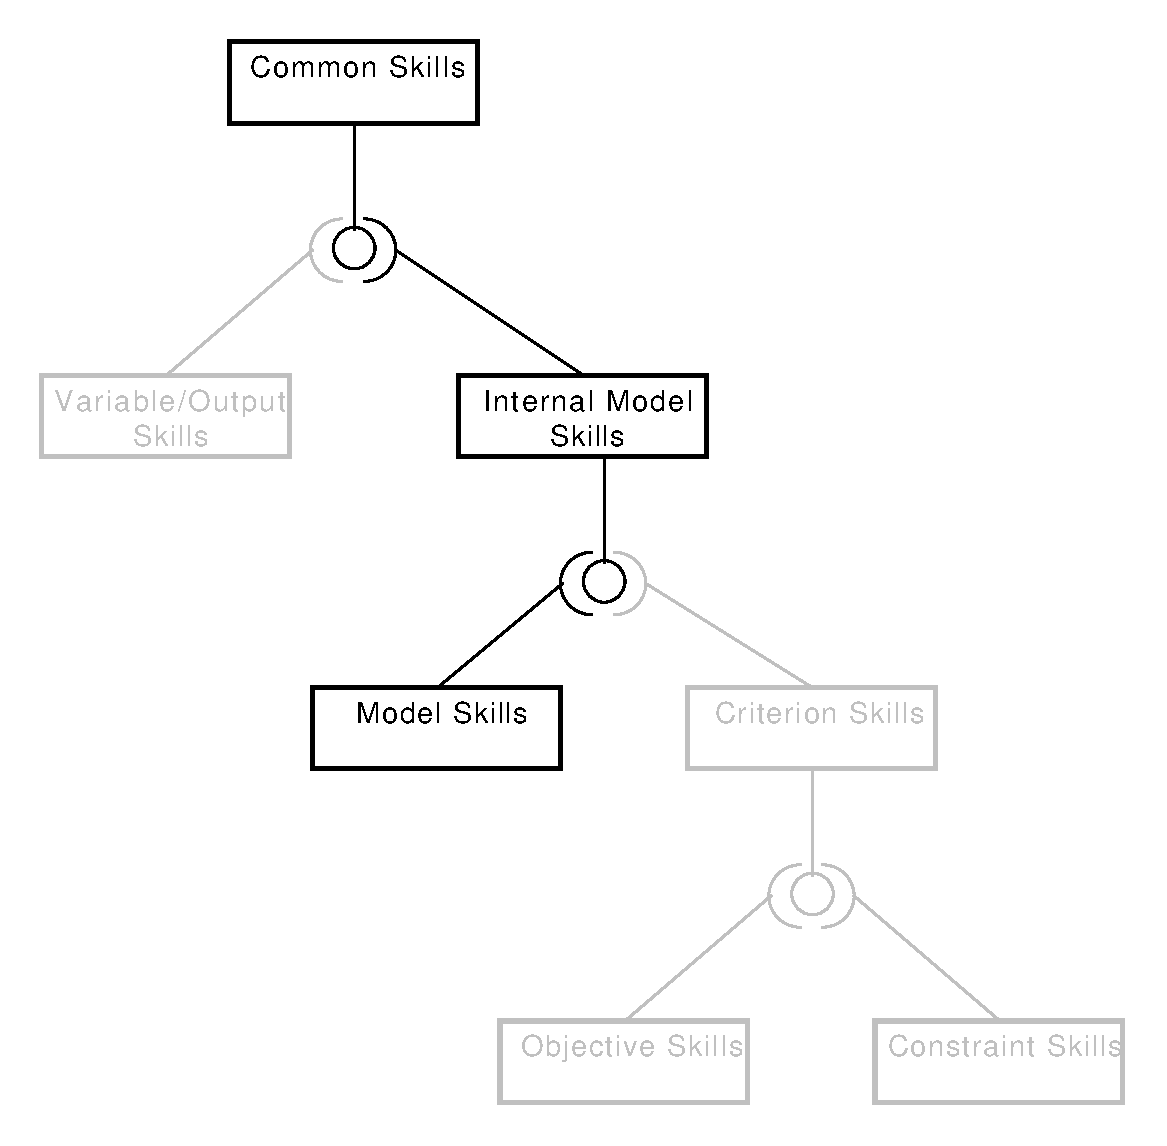
\includegraphics[width=\textwidth]{ID4CS_Speadl_skills_example}
			\caption{Model agent skills composition.}\label{skills:example}
	\end{subfigure}
\caption{\emph{Skills} component internals.}\label{skills}
\end{figure}

This tree-like structure of the skills components is not only a good way from engineering point of view a good way to factor implementation code, but is also efficient in regard of the functioning of NCS. As different NCS are shared by different agent types at different levels, this organization enables an efficient representation of [[correct ? => ]] which cooperative behavior is common to which agents. The NCS corresponding to the different components are shown in \figurename{} \ref{skills:NCS}

\begin{figure}
\centering
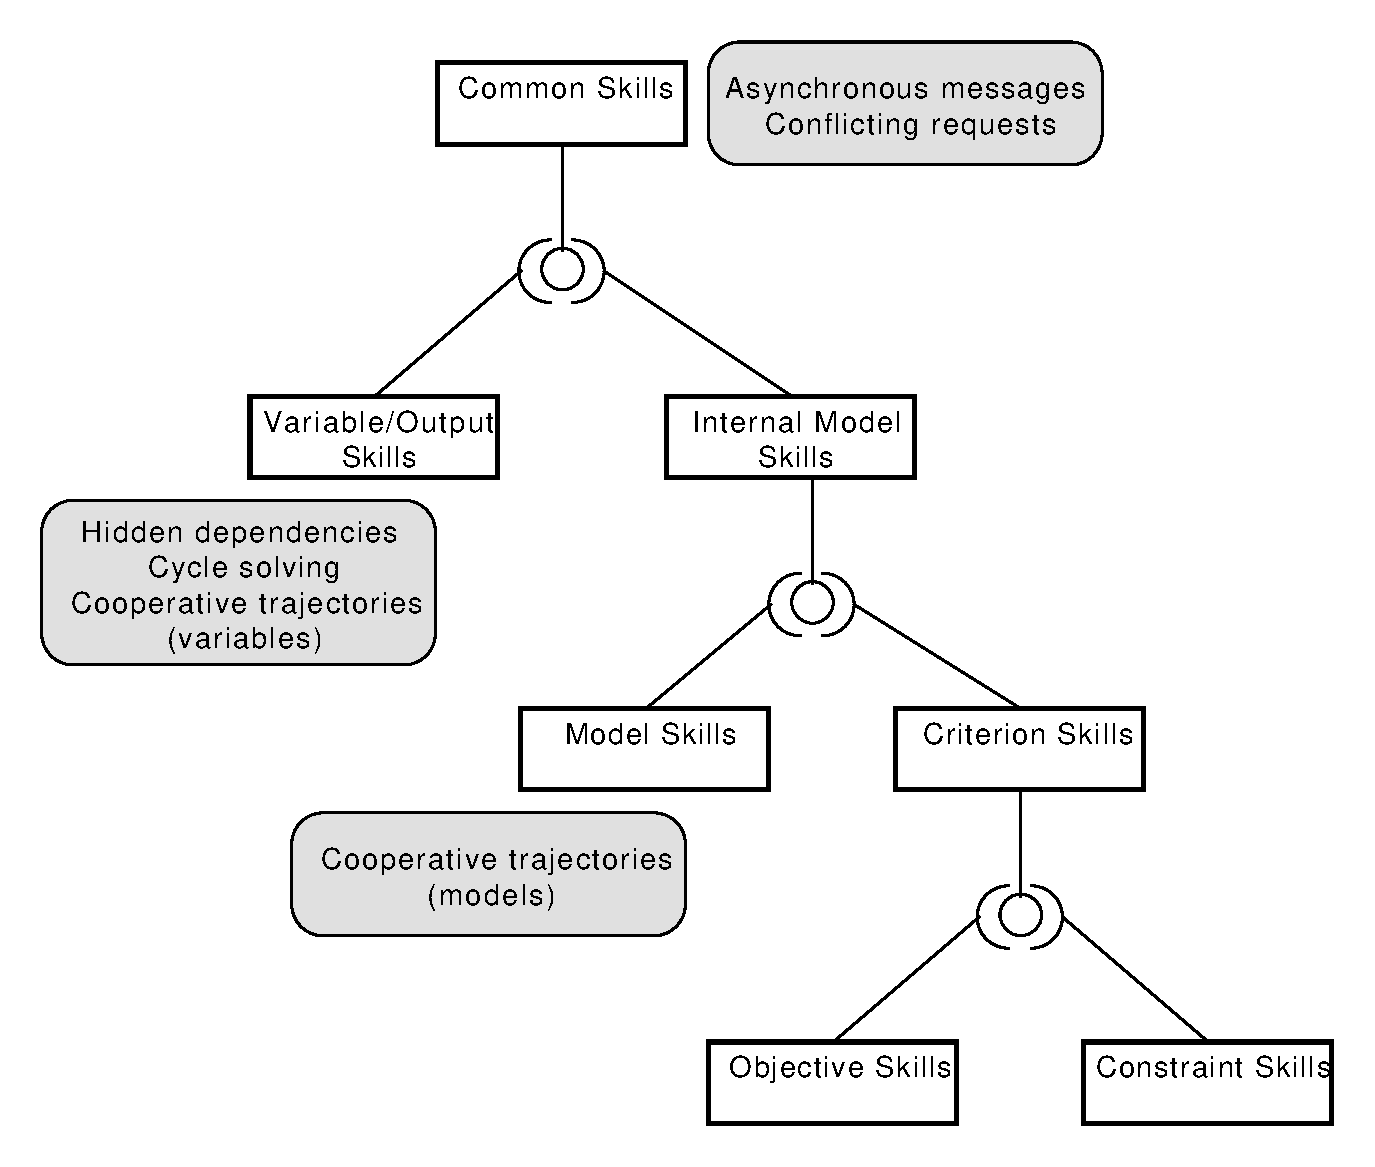
\includegraphics[width=0.6\paperwidth]{ID4CS_Speadl_skills_NCS}
\caption{Skills components dependencies tree with corresponding NCS.}\label{skills:NCS}
\end{figure}

\subsection{Communication}

The \emph{communication} view (\figurename{} \ref{Arch-comm}) presents the components related to the communication capabilities of the agent. 

\begin{figure}
\centering
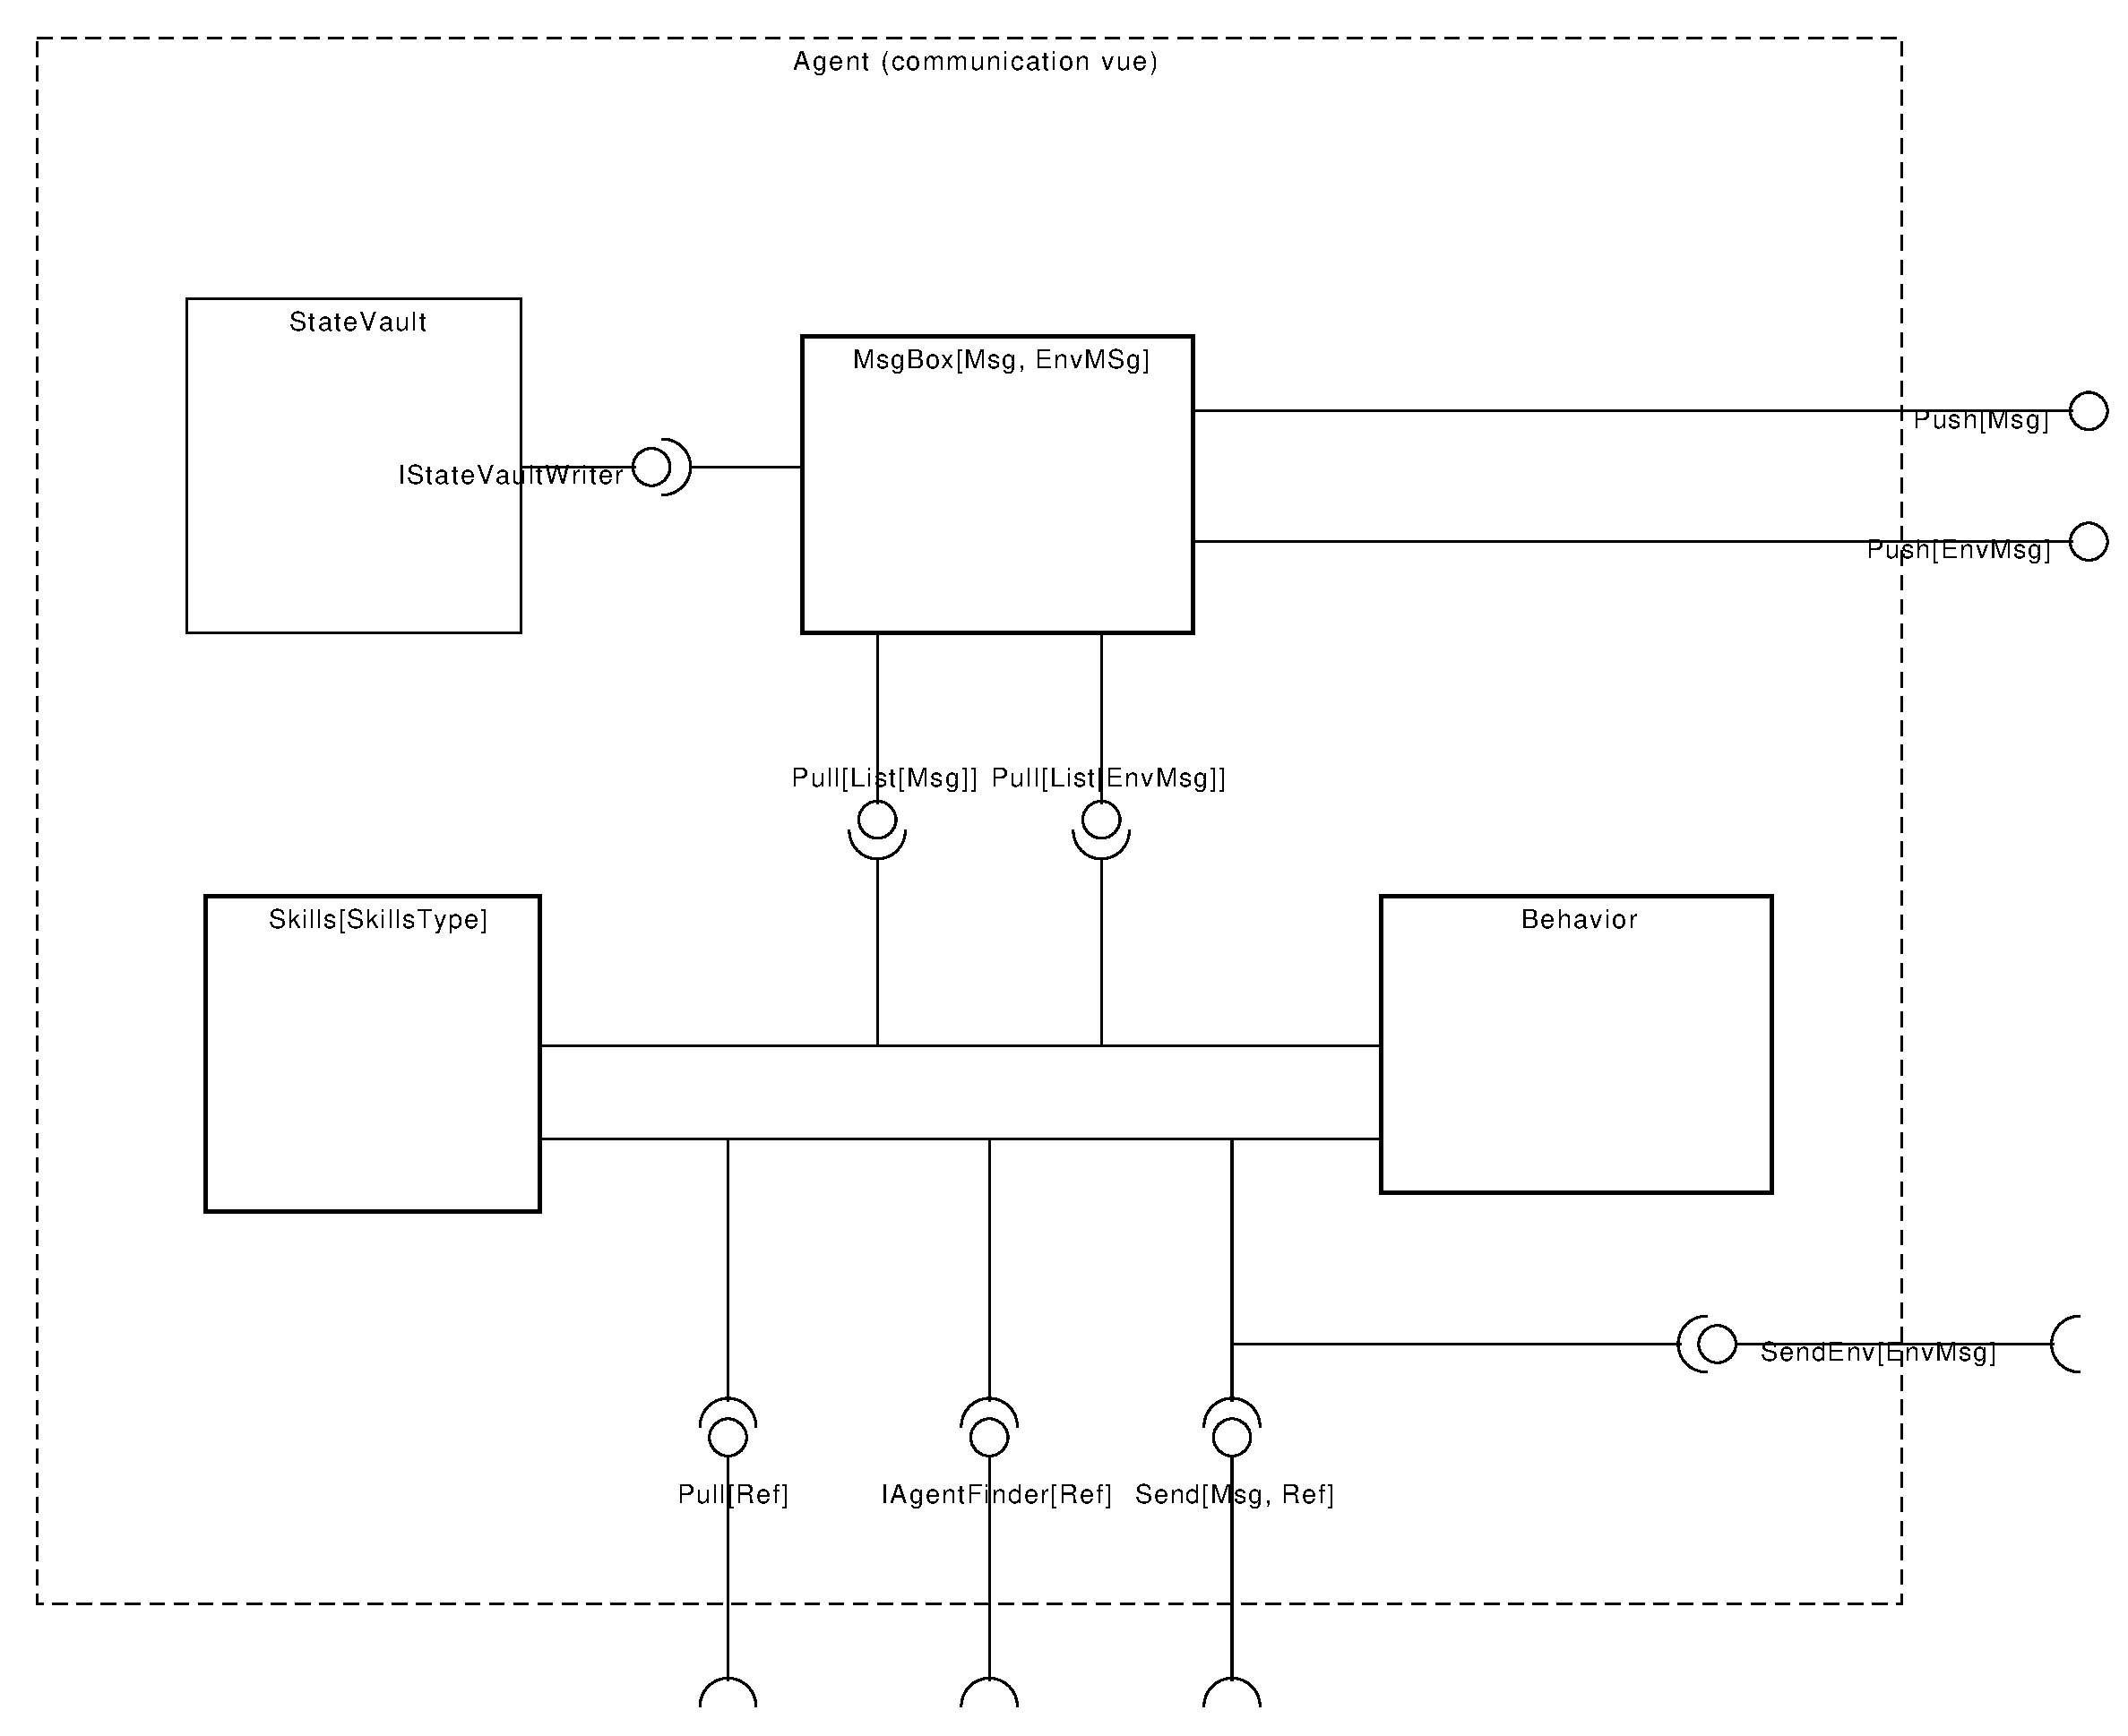
\includegraphics[width=0.6\paperwidth]{ID4CS_Speadl_comm}
\caption{Agent Architecture - Communication view.}
\label{Arch-comm}
\end{figure}

This view contains the \emph{Message Box} component, which contains the messages sent to the agent. The \emph{Message Box} stores the messages into the \emph{State Vault} and provides a direct access to the \emph{Skills} and {Behavior} components.

This figure presents several ports which need to be provided from the environment to the agent. The environment must give an unique \emph{Reference} to the agent, which will be used by the other agents to communicate with it. The environment must also provides some ports to communicate with the other agents and outside of the system.

\subsection{Monitoring}

The \emph{monitoring} view (\figurename{} \ref{Arch-monitor}) presents the components related to the monitoring of the agent. It is used to observe the agents states and their modifications.

The new component introduced in this view is the \emph{Monitor}. The \emph{Monitor} provides two ports to the environment. The first port is used for external monitoring interfaces to subscribe to be informed of changes in the state of the agent. The second is used to provide informations concerning changes of a specific part of the agent. Thus, an external monitoring interface can subscribe in order to be notified when the state of the agent changed using the first port, and then use the second port to access to the specific informations it wants to monitor.

In order to provide its capabilities, the monitor component needs to be informed by the \emph{Behavior} component before and after each step, to read and compare the monitored informations into the \emph{State Vault}.

\begin{figure}
\centering
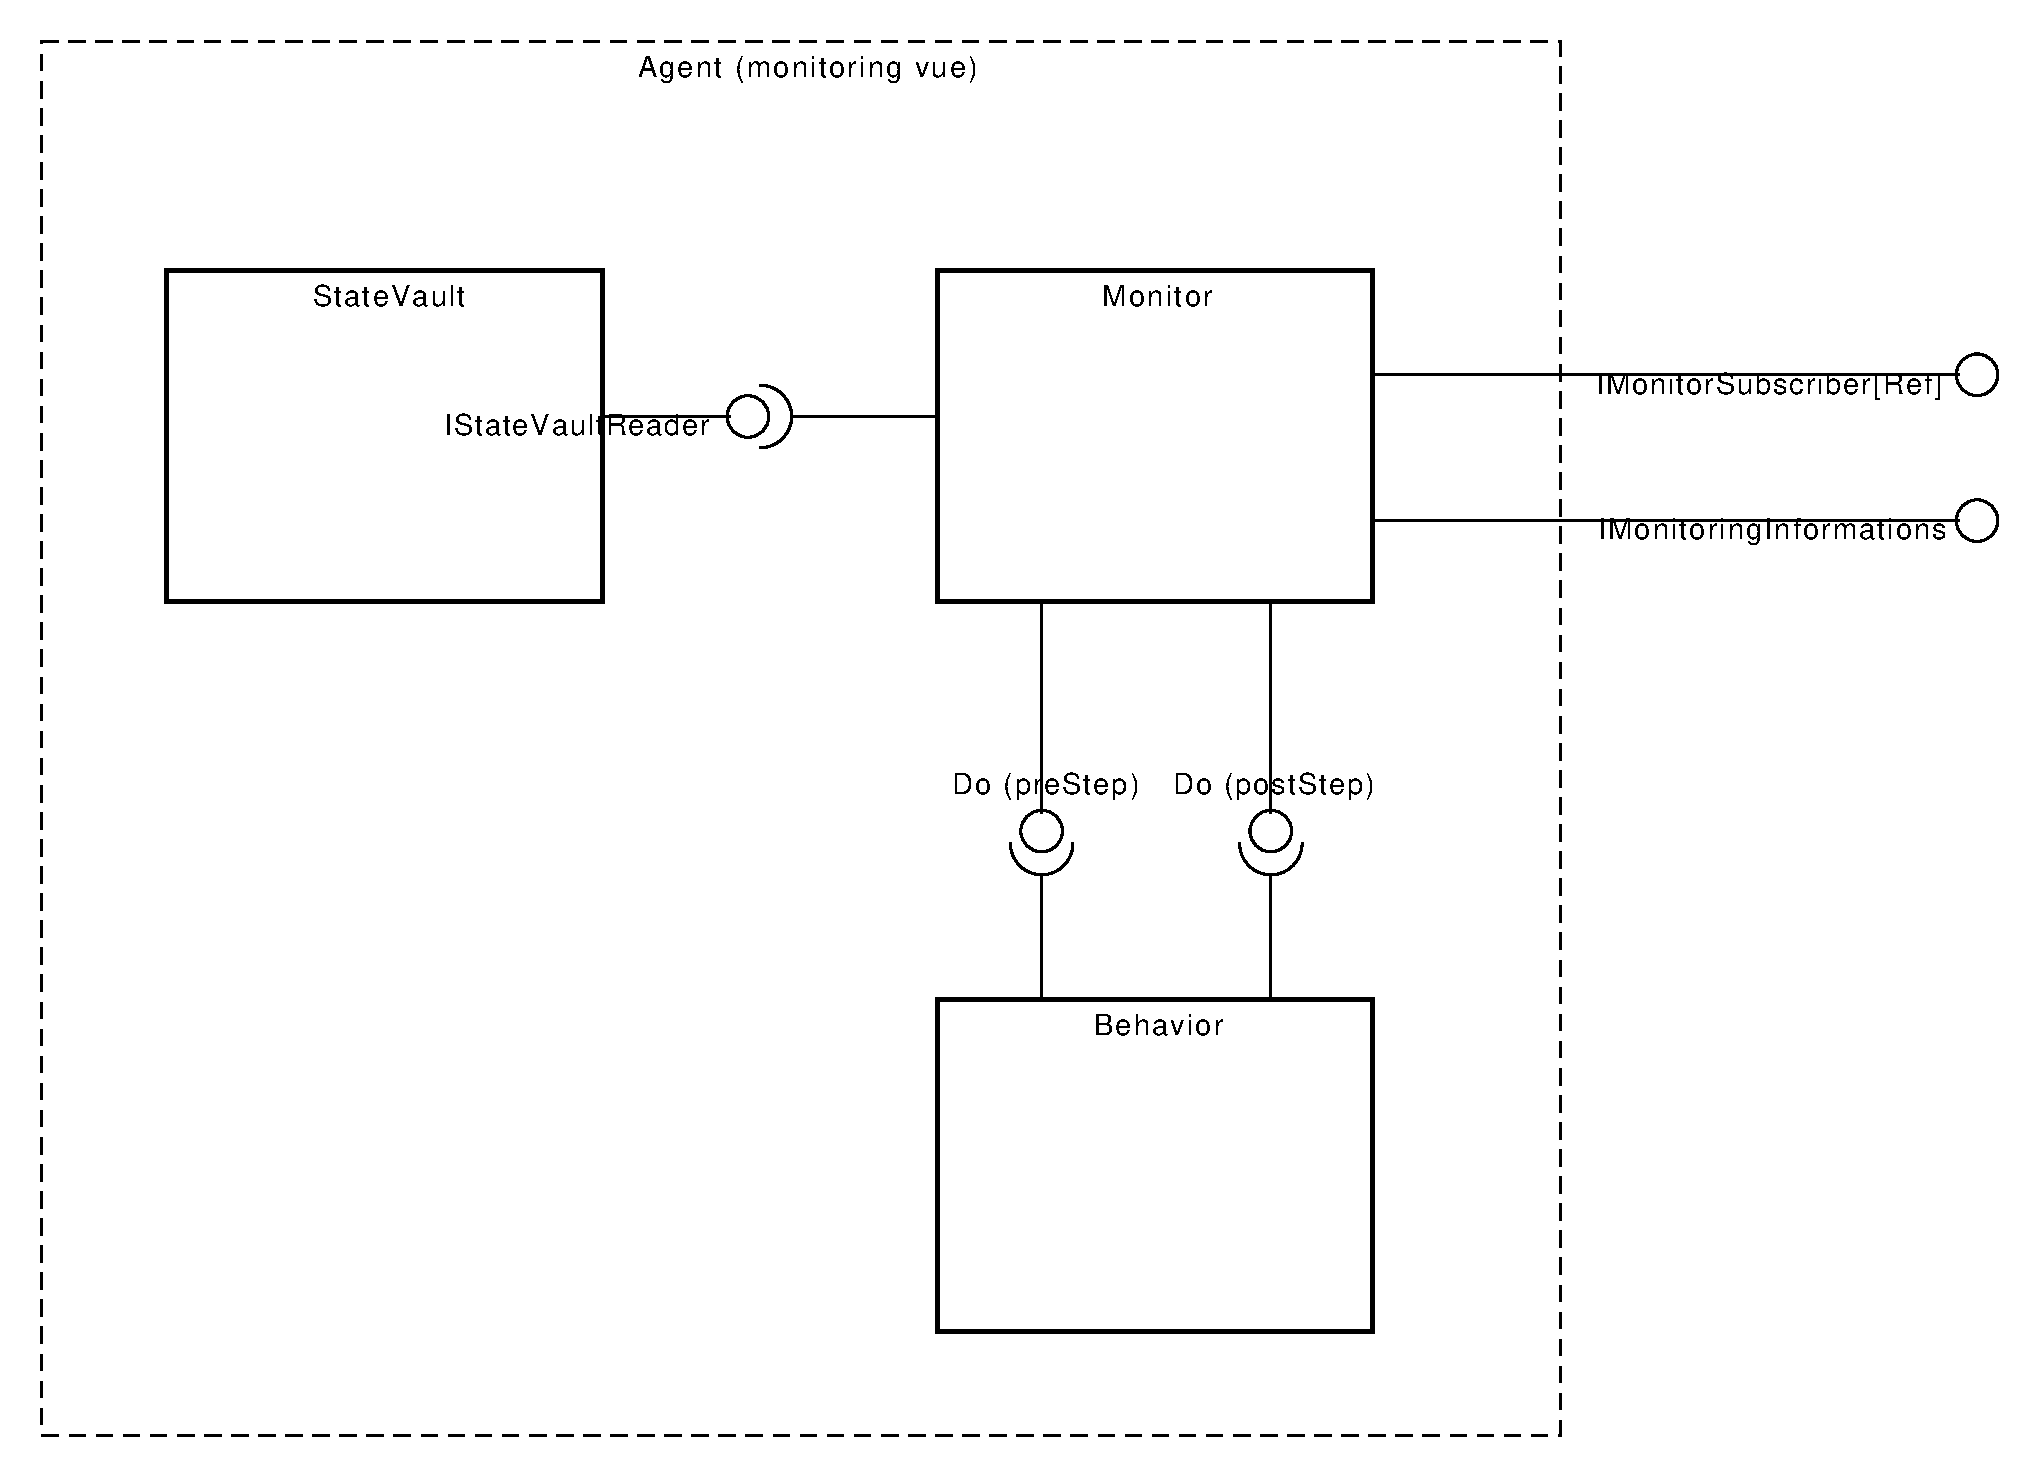
\includegraphics[width=0.6\paperwidth]{ID4CS_Speadl_monitoring}
\caption{Agent Architecture - Monitoring view.}
\label{Arch-monitor}
\end{figure}

\section{MAY MAS Architecture}

The MAY framework does not only allow to design the architecture of the agents, but can also be used to design the whole architecture of the MAS. This MAS architecture defines how the agents can interact among themselves and with their environment. Concerning our prototype, this architecture first provides support for the messages passing among the agents. The architecture of the system, which is explained below, is shown on \figurename{} \ref{Arch-MAS}.

\begin{figure}
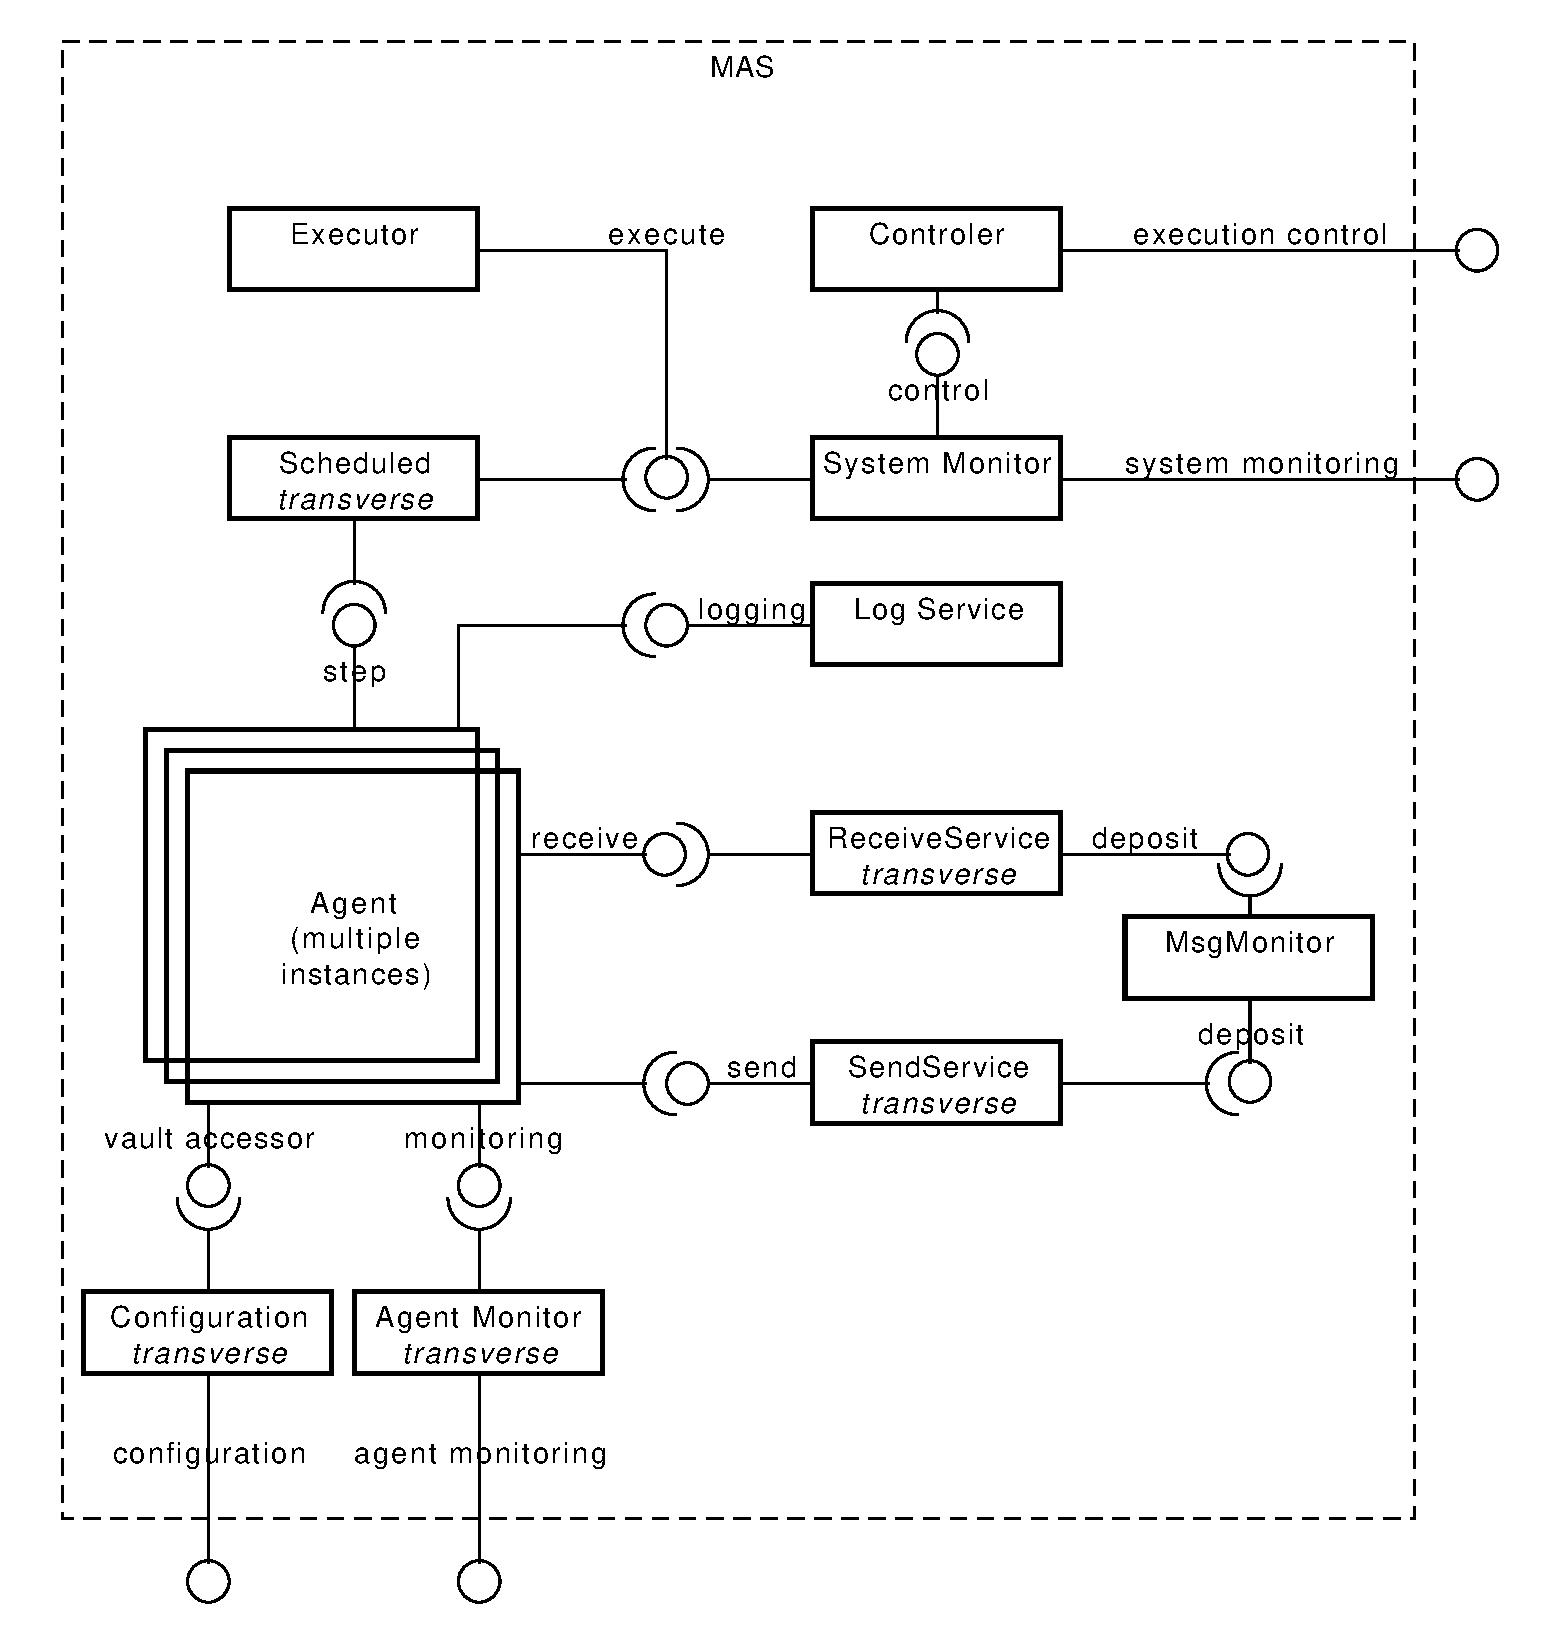
\includegraphics[width=\textwidth]{ID4CS_Speadl_system}
\caption{MAS Architecture}\label{Arch-MAS}
\end{figure}

In order to support the integration of multiple agent instances into the global system architecture, MAY provides the concept of \emph{transverse}. A transverse is a special kind of component which makes the liaison between a component on one side and multiple instances of a component on the other. The main use of transverses is to connect all agents instances to the others components of the system.

The components \emph{SendService} and \emph{ReceiveService} are MAY components used to exchange messages between the agents. While they are usually directly connected together, we inserted between them a \emph{MsgMonitor} component, which allows us to monitor the messages transmissions. The agents also have the capability to create log messages to be written into log files using the \emph{Log Service} component.

Some interfaces for configuring and monitoring the agents are exposed to the outside of the MAS through the \emph{Configuration} and \emph{Agent Monitor} transverses. The \emph{Agent Monitor} component exposes some representative information on the agents, while the \emph{Configuration} component offers a direct access to the agent state vault, allowing to examine the raw data as well as offering ways to the user to interact with the agents (changing values, constraints thresholds \emph{etc.}).

A more complex monitoring interface is provided by the \emph{System Monitor}. This component not only allows for advanced monitoring functionalities (like subscribing to changes notifications), but also handles the execution of the system though the \emph{Executor} component. The \emph{Executor} handles the low-level execution concerns, like creating threads and executing tasks, and is in charge of executing the code of the agents through the \emph{Scheduled} component. A very similar configuration (not presented on the diagram) allows the agents to exchange messages with the outside of the system. The \emph{System Monitor} is linked to a \emph{Controler} component, which is in charge of exposing a convenient execution control interface for the user or for an external program.

\section{Integration into the Prototype}

This implementation of the MAS was part of a collective development effort to provide a functional prototype. The goal of this prototype is to be a end-user aimed tool of the possibilities offered by agent-based continuous optimization.

The development of the prototype was carried mainly by three partners[[cite them?]], each in charge of a different aspect.

The prototype can be divided in three parts: The Graphical User Interface (GUI), the core module (CORE) and the Multi-Agent System (MAS). The CORE provides a common representation of the manipulated data and is in charge of maintaining consistency between the GUI and the MAS.

These three modules communicate using the OSGi framework\footnote{\url{http://www.osgi.org}}.

\subsection{MAS}

The MAS implementation is the main contribution of this thesis and was already presented in the previous parts. The only additional work was to encapsulate the implementation into an OSGi bundle which exposes the functionalities corresponding to the external services exposed by the MAS architecture and presented in the previous section.

\subsection{CORE}

The CORE module is responsible of maintaining consistency of the manipulated data. It serves as a middle-man between the MAS and the GUI. It also makes possible to enable data persistence by providing a serialization/deserialization service.

\subsection{GUI}

The GUI was build using the Eclipse Rich Client Platform (RCP)\footnote{\url{http://wiki.eclipse.org/index.php/Rich_Client_Platform}}. RCP allows to compose graphical interface components into a user interface. It was used to propose graphical tool inspired by existing development environments, providing the user with the possibility to define workspaces in which it can define problem elements which can then be used to define optimization problems.

\bigskip

By combining these three modules, we obtained a prototype which can be used to create optimization problems. To create a problem, the user can either provide a textual definition or use the graphical tools. In the last case, the user defines different reusable components (variables, models \emph{etc.}). He is then able to drag-and-drop them from an element palette on a graph canvas and to draw links between the different elements, effectively creating the problem using our NDMO graph representation. Either way, the problem is automatically translated in an instance of the MAS, which can be controlled by the user during the optimization process. A screenshot of our prototype, showing the graph canvas on which the graph of a problem is currently being created, is shown on \figurename{} \ref{tool}.

\begin{figure}
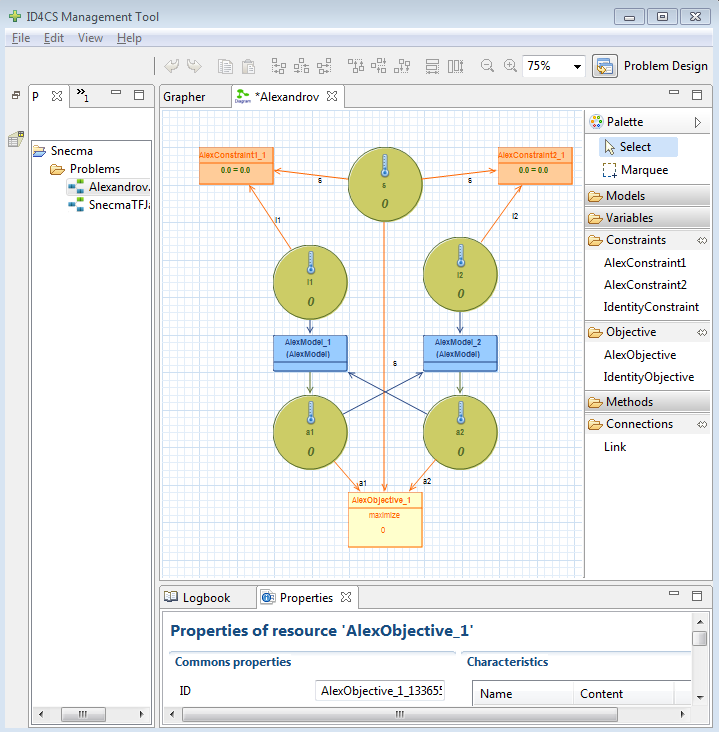
\includegraphics[width=\textwidth]{tool}
\caption{User Interface of our prototype (problem canvas view)}\label{tool}
\end{figure}